\documentclass[11pt]{book}

%\usepackage{setspace}
%\usepackage{fullpage}
%\usepackage{relsize}
\usepackage{graphicx}
\usepackage{geometry}

\usepackage[sc]{mathpazo} 	% Use the Palatino font
\usepackage[T1]{fontenc} 		% Use 8-bit encoding that has 256 glyphs
%\linespread{1.05} 			% Line spacing - Palatino needs more space between lines
\usepackage{microtype} 		% Slightly tweak font spacing for aesthetics

%\usepackage[hmarginratio=1:1,top=32mm,columnsep=20pt]{geometry} % Document margins

\usepackage[
	pdfauthor={John T. Johnson},%
	pdftitle={The PCB-GCODE User's Manual},%
	pdfsubject={pcb-gcode mechanically etching printed circuit boards},%
	pdfkeywords={pcb-gcode}{g-code}{pcb}{cnc}{etching},%
	colorlinks=true,%
	linkcolor=gray,%
	urlcolor=gray%
]{hyperref} 		% For hyperlinks in the PDF

\usepackage[hang, small,labelfont=bf,up,textfont=it,up]{caption} % Custom captions under/above floats in tables or figures
\usepackage{booktabs} 		% Horizontal rules in tables

\usepackage{paralist} 		% Used for the compactitem environment which makes bullet points with less space between them

\usepackage{fancyhdr} 		% Headers and footers
%\pagestyle{fancy} 			% All pages have headers and footers
\fancyhead{} 				% Blank out the default header
\fancyfoot{} 				% Blank out the default footer
%\fancyhead[C]{SED1 $\bullet$ December 5, 2012 $\bullet$ Unpublished} % Custom header text
\fancyfoot[RO,LE]{\thepage} 	% Custom footer text

\usepackage{varioref}

%\usepackage{lmodern}

\usepackage{listings}

\usepackage{textcomp}

\usepackage{float}

\usepackage[section]{placeins}

%\usepackage{draftwatermark}

\usepackage{makeidx}
\makeindex
%\usepackage{showidx}		% shows index items in margins, doesn't gen index page

%----------------------------------------------------------------------------------------
%	TITLE SECTION
%----------------------------------------------------------------------------------------

\title{\vspace{-15mm}\fontsize{24pt}{10pt}\selectfont\textbf{The PCB-GCODE User's Manual}\\[1em]
\fontsize{18pt}{10pt}\textsc{Version 3.6.2}\\[1em]
}

\author{
\large
Copyright \copyright\ 2014\\[1em]
\textsc{John T. Johnson}\\[2mm] %\thanks{A thank you or further information}\\[2mm] % Your name
\normalsize \href{mailto:pcbgcode@pcbgcode.org}{\texttt{pcbgcode@pcbgcode.org}} % Your email address
\vspace{-5mm}
}
%\date{} % empty date, since it is shown in the header

%\makeglossary

% Adobe bug workoround
\pdfminorversion=4

% no-break code environment to prevent page-breaking a listing
\lstnewenvironment{nbcode}[1][]%
  {\minipage{\linewidth} 
   \lstset{language=eagle,
	basicstyle=\ttfamily\small,
	numberstyle=\small\color{gray},
	numbers=left,
	showstringspaces=false,
	stepnumber=1,
%	frame=shadowbox,
	breaklines=true,#1}}
  {\endminipage}


%======================================================================
%======================================================================
\begin{document}
%======================================================================
%======================================================================

%\newcommand{\marginnote}[1]{%
%  \marginpar{\colorbox{yellow}{\parbox{\marginparwidth}{%
%  %\setstretch{0.5}
%  \textcolor{red}{\scriptsize{#1}}}}}}

\newcommand{\warning}[1]{
	\marginpar{
		\vspace{0.1in}
		\includegraphics{/Users/john/Dropbox/Docs/warning.pdf}
		\centering
		#1
	}
}

\newcommand{\information}[1]{
	\marginpar{
		\vspace{0.1in}
		\includegraphics{/Users/john/Dropbox/Docs/information.pdf}
		\centering
		#1
	}
}

\newcommand{\howitworks}[1]{
	\marginpar{
		\vspace{0.1in}
		\includegraphics{/Users/john/Dropbox/Docs/gears.pdf}
		\centering
		#1
	}
}


  
\setlength{\marginparwidth}{1.0in}
\setlength{\marginparsep}{1em}


\newcommand{\code}[1]{\texttt{#1}}

\definecolor{gray}{rgb}{0.5,0.5,0.5}

\lstset{language=eagle,
	basicstyle=\ttfamily\small,
	numberstyle=\small\color{gray},
	numbers=left,
	showstringspaces=false,
	stepnumber=1,
%	frame=shadowbox,
	breaklines=true}

\frontmatter

\maketitle

%
%---------------------------------------------------------------------
%
\section*{About this book}

This book is typeset with \href{http://en.wikipedia.org/wiki/LaTeX}{\LaTeX{}} using the Computer Modern and Palatino fonts.
\vspace{1ex}

\noindent The \LaTeX{} distribution used is \href{http://tug.org/mactex/}{MacTeX}. The editor is \href{http://texpadapp.com}{Texpad} for \href{http://www.apple.com/osx/}{Mac OS X} and \href{http://www.apple.com/ios/}{iOS}. When doing academic writing, I use \href{http://bibdesk.sourceforge.net}{BibDesk} on Mac OS X and \href{https://itunes.apple.com/us/app/pocketbib-for-bibtex-bibdesk/id524521749?mt=8}{PocketBib} on iOS.
\vspace{1ex}

\noindent Some words, such as MacTeX in the previous paragraph, are links to websites. In this manual, all links are colored gray. The reader will note that other words are links to figures, tables, or sections in this manual. These are also colored gray.
\vspace{1ex}

\noindent Throughout this book there are icons in the margins that will help the reader navigate the book and find material at an appropriate skill level. These icons are shown below.
\vspace{1ex}

\howitworks{} \noindent Sections marked with this icon provide background on the operation of pcb-gcode. This information is for curious users and can safely be skipped.
\vspace{7ex}

%\information{} \noindent Information.
%\vspace{10ex}

\warning{} \noindent Some parts of the manual are for intermediate or advanced users. This icon alerts the reader to this fact.

\vspace{2ex}

\newpage

\section*{Supporters}

\noindent There is a great community that has built up around pcb-gcode where users freely offer advice and help solve problems for other users. Despite the fact that pcb-gcode has always been free and always will be, a few outstanding individuals have donated time or money (which goes towards paying for web hosting for \url{pcbgcode.org}). Your generosity warms my heart, and I thank you all!

\begin{itemize}
	\item Art Eckstein is the tireless moderator of the Yahoo! group.
	\item Translations
	\begin{itemize}
		\item Maur\'icio Dias --- Portugu\^ese
		\item Wolfgang Schmidt --- German
	\end{itemize}
	\item{Monetary Donations (If I missed you, \emph{please} let me know.) }
	\begin{itemize}
    	\raggedright
		\item Anonymous (2007), Greg Brill, Paul Kiedrowski, Steven Manzer, Barry Ward, Ward Elder, Art Eckstein, World of ElectroMechanica, Austin~Valley~Software~Corporation, webstudio.co.uk, Juan Posada, Richard~McCarthy, Keeley~Electronics
	\end{itemize}
	\item{Code Contributions}
	    \begin{itemize}
	    \small
	    \item Martin L. Marriott - G-code optimizer
	    \item Peter Zotov - Stencil generation for cream layers
	    \end{itemize}
	\item{Beta Testers}
	\begin{itemize}
    	\raggedright
	    \item Art Eckstein, Astrid Adam, Brett Pound, Danny Miller, Juan Posada, Martin~Marriott, Maur\'icio Dias, Svend Poulsen, Zulfqar Ali.
	\end{itemize}
\end{itemize}


\tableofcontents

\listoffigures

\listoftables

\mainmatter

%======================================================================
%
\chapter{Introduction}\label{chp:Introduction}
%
%======================================================================

%
%---------------------------------------------------------------------
%
\section{Purpose}\label{sec:Purpose}

Pcb-gcode is a User Language Program (ULP) for EAGLE PCB design software produced by \href{http://cadsoftusa.com}{CadSoft}. Pcb-gcode allows one to make printed circuit boards by using a CNC router or milling machine to cut the traces out of the copper on the board. It also produces files for drilling holes and creating stencils for cream layers. Two-sided boards are supported. By "mechanically etching" the boards, no toxic chemicals are needed -- making the process more environmentally friendly. Turn-around times and costs are much reduced from ordering a prototype from a board house.

%
%---------------------------------------------------------------------
%
\section{Features}\label{sec:Features}

Though no program can be all things to all people, pcb-gcode has a lot of features to help make it useful.

\begin{description}
	\item[One or two sided boards] There are checkboxes for selecting whether to generate files for the top and/or bottom sides of the boards.
	\item[Outlines] Generate gcode for cutting around the tracks of the PCB. Multiple passes are possible, which helps eliminate the small slivers that may be left behind. There is also an option to make only one outline pass.
	\item[Drills] Generate gcode for drilling component and mounting holes. Tool changes are supported, as well as a drill rack file.
	\item[Preview] A preview for outlines is available.
	\item[Milling] Milling code can be generated for any wires drawn on the Milling (46) layer.
	\item[Text] Generates gcode to engrave any vector text that is on the Milling (46) layer.
	\item[Stencils] Produce stencils for applying solder cream for surface-mount parts.
	\item[Spot drill holes] Holes can be spot drilled with the outlines tool to help the drill bits to start straight when drilling holes.
	\item[Tool change position] Where the machine should go so that the tool can be changed.
	\item[Drill rack files] Allows using one drill bit for a range of hole sizes in the board.
	\item[Profile] Starting settings for particular styles of gcode, for example, Mach3 or EMC, among others.
	\item[Embedding comments] Comments documenting the settings a file was created with can be inserted into the gcode.
	\item[User gcode] For users that need to generate gcode for unusual situations.
	\item[File naming] Several options exist for naming files according to the conventions of the user's controller, and their local language.
	\item[Plugins] Allow for future expansion.
\end{description}

%
%---------------------------------------------------------------------
%
\section{How it Works}\label{sec:HowItWorks}
\subsection{Overview}
After designing your board in Eagle's board editor, the ULP \code{pcb-gcode-setup} is run and options are set (See \figurename \vref{fig:SetupGenerationOptions}). Pcb-gcode will generate a set of files that will cut out the tracks, pads, pours and vias (hereinafter called tracks) for the top and/or bottom of the board. Pcb-gcode can also generate files to drill holes from the top and/or bottom of the board. Since the holes usually go all the way through, they only need to be drilled from one side, although some users have drilled slightly more than half way from both sides for a cleaner finish. The user may also choose to create milling wires on the milling layer of the board. This can be used to cut out sections of the board, or cut the perimeter of the board out. There is also an option for engraving vector text that the user places on the milling layer.

After the files are generated, they are transferred to the control software for the CNC router or milling machine. The PCB is mounted on the machine. The origin is set to the lower left for the top side of the board and the top files are run. The board is then flipped in the \code{X} axis (i.e. around the \code{Y} axis), the origin is set at the lower right, and the bottom files are run. After minimal inspection and cleanup, the board is ready to be loaded with components.

\subsection{Isolation}\index{isolation!description}
Pcb-gcode has the ability to generate g-code that cuts out tracks with increasing amounts of isolation. This is helpful because it can help eliminate small slivers of copper left behind by the cutting process.

The isolation begins at a minimum amount and is increased by a step size until a maximum amount is reached. The builtin previewer can be used to see how this isolation works. See \figurename \vref{fig:MultipassBoard}. From the zoomed view shown in \figurename \vref{fig:MultipassBoardZoom} you can see that the passes start out close to the track, then move out by a step size. The colors of the preview tracks follow the standard resistor color codes, so brown is the first pass, red is the second, orange the third, etc.

\howitworks{}
For the curious reader, the isolation is calculated as shown in Equation \vref{egn:IsolationCalculation}. You do not need to know this to use pcb-gcode. Note that this formula is erroneous and that the $EtchingToolSize$ should be divided by 2 to yield the offset. Changing this now would break many user's setups, so it will be left as is. Most users arrive at the setting for the etching tool size by trial and error, so it is likely a moot point.

\begin{equation}
isolation = EtchingToolSize+MinimumIsolation+PassNumber*StepSize
\label{egn:IsolationCalculation}
\end{equation}


\begin{figure}
	\center{
	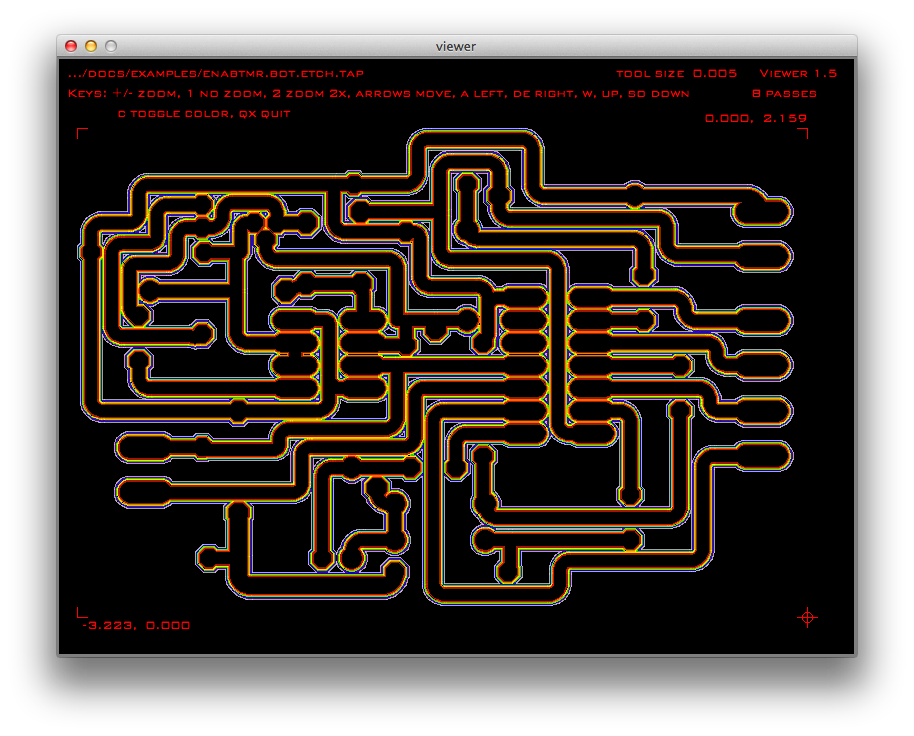
\includegraphics[width=10cm]{figs/Multipass-Board.png}
	}
	\caption{Preview showing color-coded multiple passes.}
	\label{fig:MultipassBoard}
\end{figure}

\begin{figure}
	\center{
	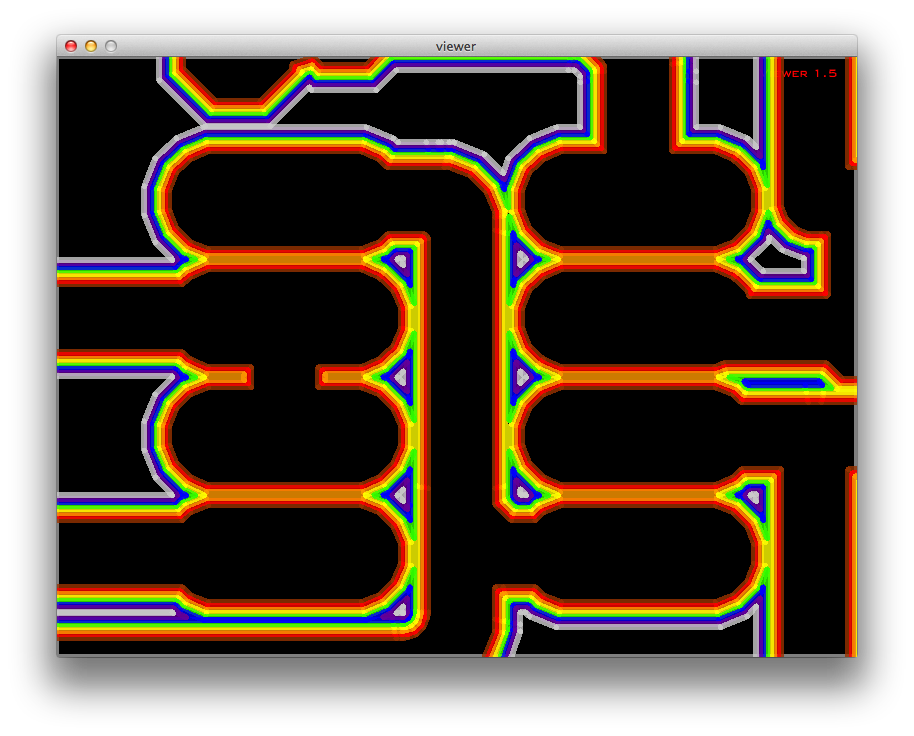
\includegraphics[width=10cm]{figs/Multipass-Board-Zoom.png}
	}
	\caption{Preview showing a zoomed version of the color-coded multiple passes. Brown is the first pass, red the second, orange the third, etc.}
	\label{fig:MultipassBoardZoom}
\end{figure}

\subsection{Drilling}\index{drill!description}
Compared to the isolation passes and files, drill file creation is relatively straight forward. Each hole in the board is sorted according to size and distance from other holes of the same size. G-code is created to position and drill each hole. Tool changes can be included in the file so that the user or an automated tool changer can change the bit. Optionally a rack file can be used. 

Rack files contain a list of drills the user has available and the size holes they can be used for. For example, if a library part has a 1mm hole, and another part has a 1.1mm hole, a 1.1mm drill bit could be used for both. For more information on rack files, see Section \vref{sec:DrillRackFiles}. 

%======================================================================
%
\chapter{Setup}\label{chp:Setup}
%
%======================================================================

%
%---------------------------------------------------------------------
%
\section{EAGLE compatibility}\label{sec:EAGLECompatibility}\index{compatibility!eagle}

Pcb-gcode is compatible with EAGLE versions 5 and 6\footnote{CadSoft changed the way numbers were represented internally with their release of version 6. This effectively broke parts of pcb-gcode. Version 3.6 incorporates changes for compatibility with version 5 or 6.}. For versions of EAGLE before version 5, pcb-gcode version 3.3.3 is still available \href{http://groups.yahoo.com/group/pcb-gcode/files/\%21\%20Software/pcb-gcode-3.3.3.zip}{in the Yahoo! group}. This manual does not apply to version 3.3.3. Please see the documentation included with version 3.3.3.
%
%---------------------------------------------------------------------
%
\section{Installation}\label{sec:Installation}\index{installation}

\subsection{Downloading and unarchiving}
Pcb-gcode can be downloaded from the Yahoo! group's \href{http://groups.yahoo.com/group/pcb-gcode/files/\%21\%20Software}{software folder}. \index{download site} Unzip the archive into a place where the operating system will allow files to be saved. For Windows, this should be somewhere inside your Documents\footnote{For Windows XP: "C:\textbackslash{}Documents and Settings", for Windows 7: "C:\textbackslash{}Users\textbackslash{}[yourname]\textbackslash{}My Documents" } folder. For Mac OS X, it could be, for instance, \code{\textasciitilde/Documents/Eagle/pcbgcode}, and for Linux, somewhere off your home folder. Be sure to preserve the directory structure in the archive. See \figurename \vref{fig:folderstructure}.

\begin{figure}
	\center{
	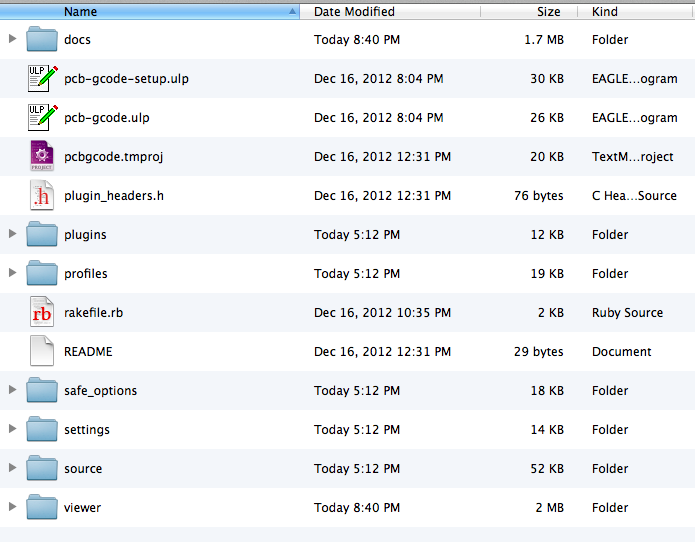
\includegraphics[width=10cm]{figs/Folder-Structure.png}
	}
	\caption{The proper directory structure after uncompressing the archive.}
	\label{fig:folderstructure}
\end{figure}

\subsubsection{Windows Note}
Note that if you are using Windows, odd things might happen if you install pcb-gcode outside the Documents folder. This is due to \href{http://en.wikipedia.org/wiki/Windows_File_Protection}{Windows File Protection} or \href{http://en.wikipedia.org/wiki/Windows_Resource_Protection}{Windows Resource Protection}, which try to keep files outside the Documents folder from being changed. This could result in, for instance, the previewer always showing the same preview or an \code{Illegal phase 0 in main routine} error\index{Error!Illegal phase 0}. If you install outside the Documents folder and have trouble, try installing under your folder inside Documents. \index{Windows File Protection}

\subsection{Configuring EAGLE}
Now that pcb-gcode is uncompressed, Eagle must know where it is located. In Eagle's \code{Control Panel}, click \code{Options $|$ Directories}, then put the path to pcb-gcode in the \code{User Language Programs} field. See \figurename \vref{fig:EagleOptionsDirectories}.

\begin{figure}
	\center{
	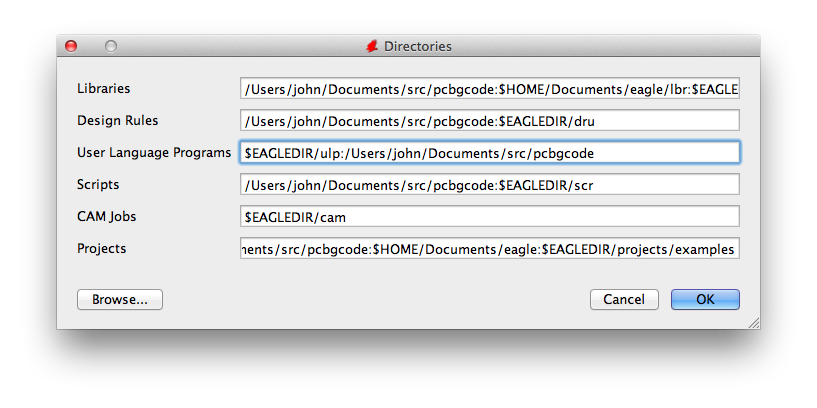
\includegraphics[width=10cm]{figs/Eagle-Options-Directories.png}
	}
	\caption{Add the path to pcb-gcode to the User Language Programs option.}
	\label{fig:EagleOptionsDirectories}
\end{figure}

\subsection{Selecting g-code style}\label{sub:SelectingGCodeStyle}\index{g-code!style}
To complete the setup, pcb-gcode must be told which type of g-code it should generate. Open a board in Eagle, then click \code{File $|$ Run...}. Locate the folder where pcb-gcode is and select pcb-gcode-setup.ulp. You will see the screen in \figurename \vref{fig:SelectGcodeStyle}. Select the style g-code that most closely matches your controller.

You will receive the warning shown in \figurename \vref{fig:GcodeDefaultsWarning}. If this is the first time pcb-gcode has been run, just click Yes and skip the rest of this paragraph. If this is an existing installation of pcb-gcode and gcode-defaults.h has been modified, make note of the modifications before clicking Yes, then make those modifications as needed to the new gcode-defaults.h file.

\begin{figure}
	\center{
	\includegraphics[width=10cm]{figs/Setup-Gcode-Style.png}
	}
	\caption{Select the style g-code pcb-gcode should produce.}
	\label{fig:SelectGcodeStyle}
\end{figure}\index{setup tabs!GCode Style}

\begin{figure}
	\center{
	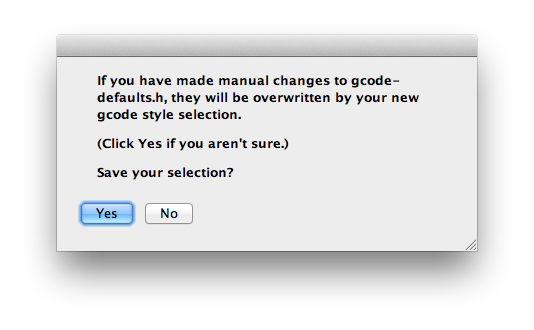
\includegraphics[width=10cm]{figs/Gcode-Defaults-Warning.png}
	}
	\caption{Overwrite warning for gcode-defaults.h.}
	\label{fig:GcodeDefaultsWarning}
\end{figure}

After clicking Yes, \code{pcb-gcode-setup} will be run again, and you will see the screen shown in \figurename \vref{fig:SetupGenerationOptions}.

\subsection{Previewer Setup}

The previewer (See section \vref{sec:Previewer}) is written in \href{http://www.processing.org}{Processing} and requires javaw.exe to run. You can download a Java runtime environment (JRE) at \href{http://www.java.com}{java.com}. You will find installation instructions there. Windows note: for the previewer to work properly, javaw.exe must be in the system path. \index{javaw.exe}\index{Java}

If you choose not to use the previewer, simply turn it off. See \figurename \vref{fig:SetupGenerationOptions}.



%
%---------------------------------------------------------------------
%
\section{Machine Setup}\label{sec:MachineSetup}

\begin{figure}
	\center{
	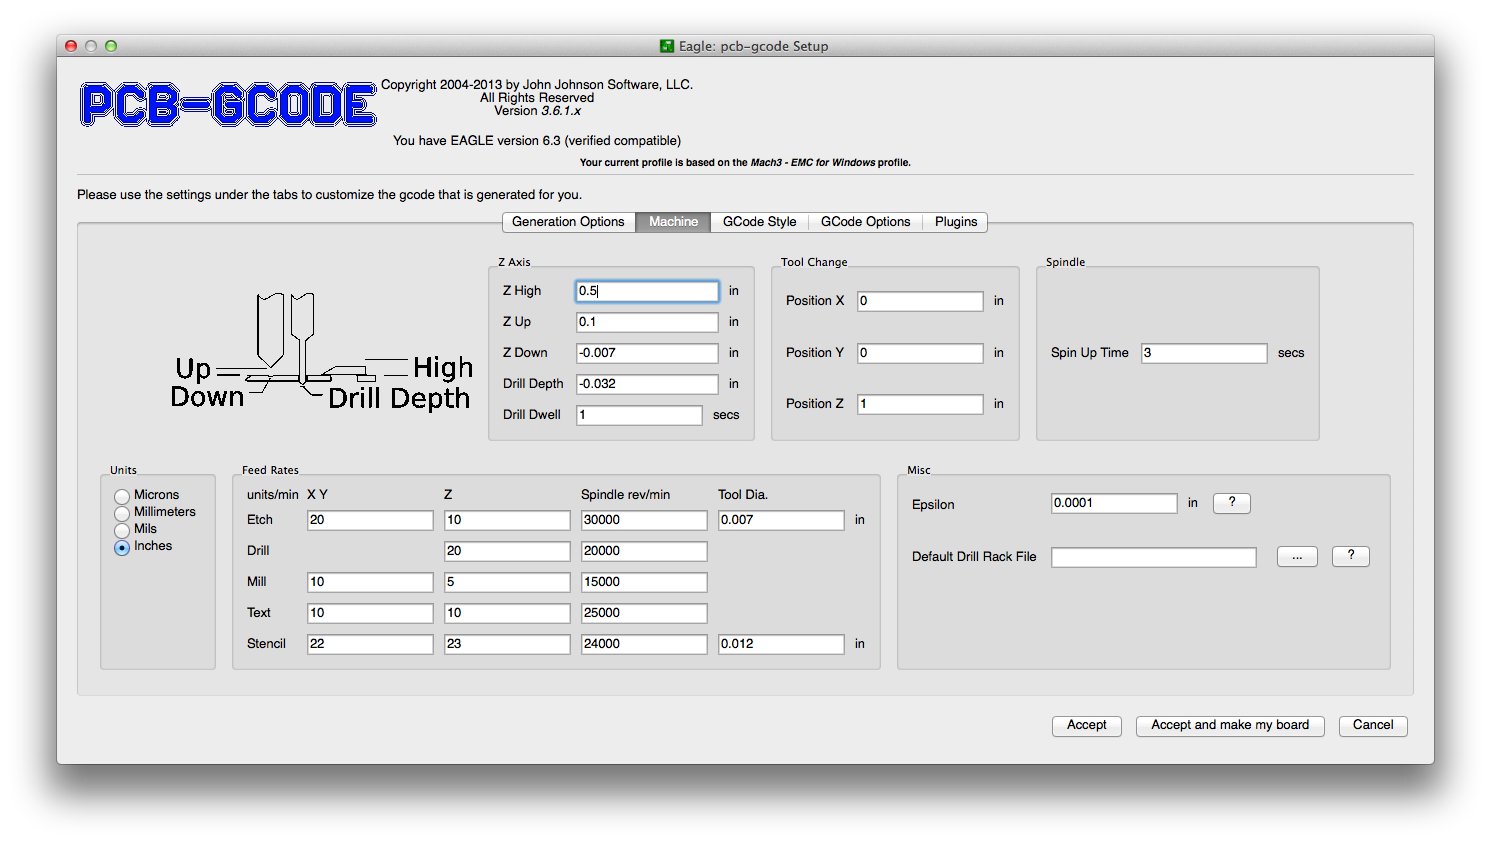
\includegraphics[width=14cm]{figs/Setup-Machine.png}
	}
	\caption{Machine options.}
	\label{fig:SetupMachine}
\end{figure}\index{setup tabs!Machine}

Click the \code{Machine} tab to view the machine options as shown in \figurename \vref{fig:SetupMachine}. First select the preferred unit of measure by selecting it under \code{Units}. \index{unit of measure}

Now set the settings for the Z axis. \code{Z High} should be high enough to clear any clamps or fixtures that hold the PCB down.\index{z axis!high} Set \code{z up} high enough to clear the board when moving from location to location.\index{z axis!up} Set \code{Z Down} to the depth into the board that the tool should cut when etching.\index{z axis!down} \code{Drill Depth} should be set deep enough to drill through the PCB.\index{drill!depth} \code{Drill Dwell} is the time, in seconds, that the drill should pause at the bottom of the hole.\index{drill!dwell}

The \code{Tool Change} options are the position where the tool should be moved when a new tool is required.\index{tool change!position}

The \code{Spin Up Time} in the \code{Spindle} box should be set to the length of time in seconds that it takes the spindle to come up to speed. If the spindle is manually controlled, this can be set to \code{1}.\index{spindle!spin up time}

The \code{Feed Rates} should be set for \code{X Y} moves as well as \code{Z} moves. Rates here will usually be quite low unless the machine has a very fast spindle. See a machinist's reference on how to calculate the optimal feed rate, use trial and error, or post to the Yahoo! group email list for advice. Note that there are separate feed rates for \code{X Y}, and \code{Z}, and there is a spindle speed setting for each of the four operations pcb-gcode can generate files for.\index{feed rates}\index{z axis!feed rates}

A \code{Tool Dia.} parameter is available to set the diameter of the tool used to etch and for milling openings for stencils used to apply cream solder paste when surface mounted parts are used.\index{stencil!tool diameter}\index{etching!tool diameter}

\code{Epsilon} is the minimum move that will be written to the g-code file. For instance, if \code{Epsilon} is set to $0.0001''$ then the g-code file will not contain movements less than $0.0001''$. This option will rarely need to be changed.

The \code{Default Drill Rack File} option allows for the selection of a rack file to be used if one has not been setup for a particular board. In most cases this can be left blank to start with. See Section \vref{sec:DrillRackFiles} for more information about setting up rack files. 

%
%---------------------------------------------------------------------
%
\section{Generation Options}\label{sec:GenerationOptions}

\begin{figure}
	\center{
	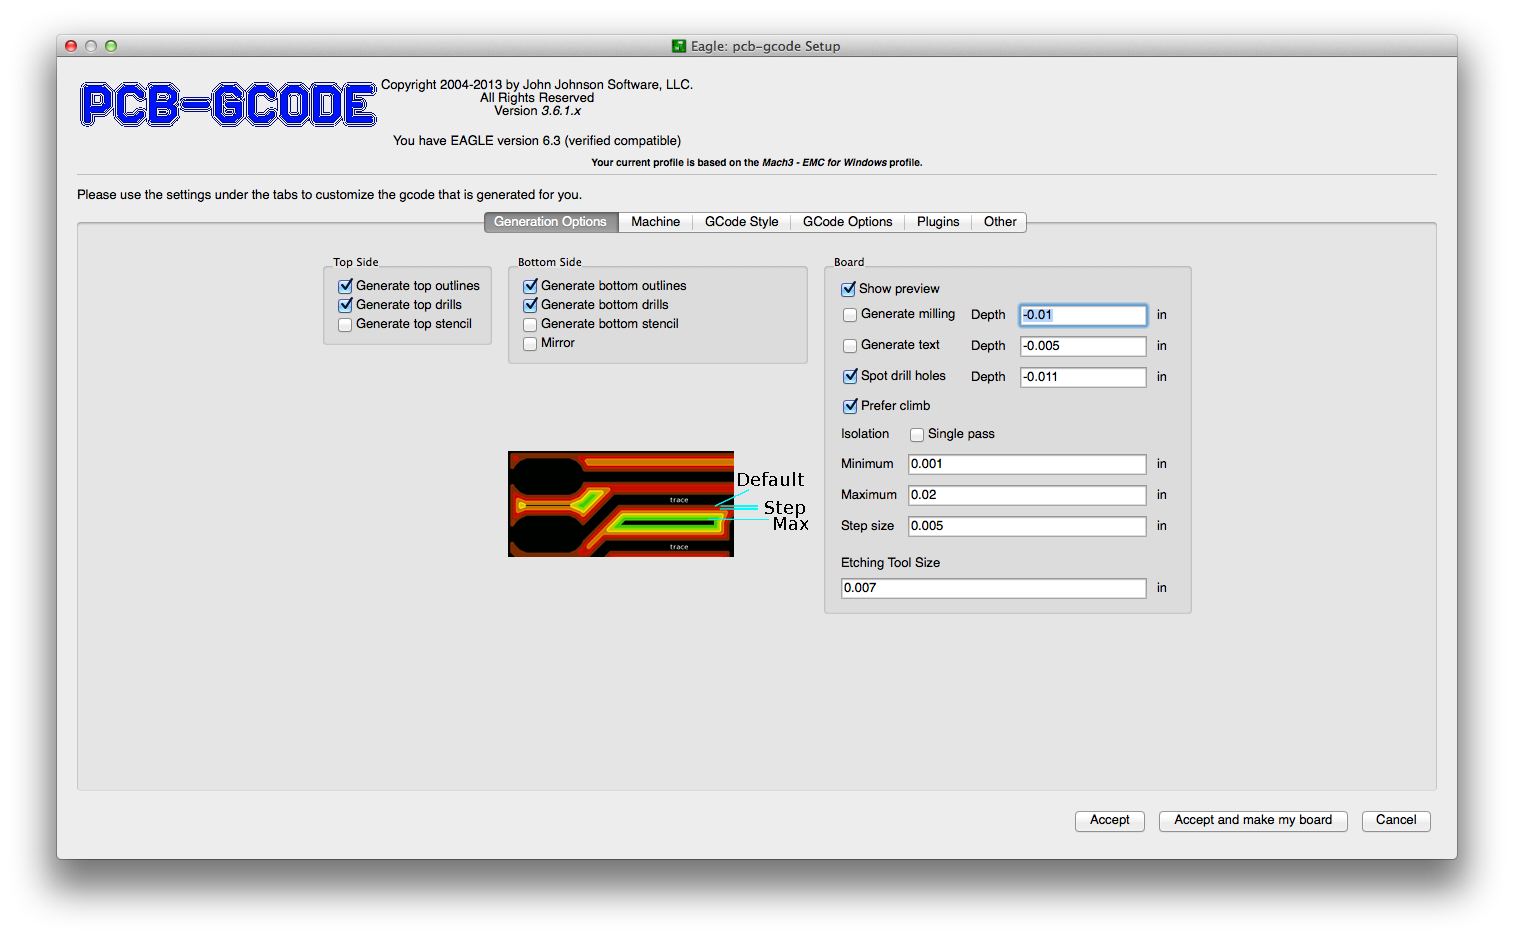
\includegraphics[width=14cm]{figs/Setup-Generation-Options.png}
	}
	\caption{Options available when generating a board.}
	\label{fig:SetupGenerationOptions}
\end{figure}\index{setup tabs!Generation Options}

Now that reasonable values have been set for the machine, click the \code{Generation Options} tab (See \figurename \vref{fig:SetupGenerationOptions}). This is where the various files produced by pcb-gcode can be selected, and common options can be set. A description of the options follows:

\begin{description}
	\item[Top Side] Options having to do with the tracks on the top of the board, and drill holes made from the top side of the board.
	\begin{description}
		\item[Generate top outlines] Generate g-code to cut out the tracks, pads, pours and vias on the top side of the board.
		\item[Generate top drills] Generate g-code to drill holes from the top side of the board.
		\item[Generate top stencil] Generate g-code to cut out a stencil for the top cream layer.\index{stencil!Generate top option}
	\end{description}
	\item[Bottom Side] Options having to do with the tracks on the bottom of the board, and drill holes made from the bottom side of the board.
	\begin{description}
		\item[Generate bottom outlines] Generate g-code to cut out the tracks, pads, pours and vias on the bottom side of the board.
		\item[Generate bottom drills] Generate g-code to drill holes from the bottom side of the board.
		\item[Generate bottom stencil] Generate g-code to cut out a stencil for the bottom cream layer.\index{stencil!Generate bottom option}
		\item[Mirror] X coordinates for the bottom of the board are usually negative. This makes setting the origin for a two-sided board easier. Turning this option on causes the X coordinates to be positive, however, the bottom tracks will be a mirror image of what they should be. So in general, leave this option off.
	\end{description}
	\item[Board] Options that apply to the board in general.
	\begin{description}
		\item[Show preview] Use the previewer in pcb-gcode to preview the g-code generated.
		\item[Generate milling] Generate g-code for any wires the user has drawn on the \code{Milling} (46) layer. \code{Depth} sets the milling depth.
		\item[Generate text] Generate g-code to engrave any vector text the user may have placed on the \code{Milling} layer. \code{Depth} sets the engraving depth. Not that text on the top or bottom layers will be outlined just as the tracks are, whereas text on the milling layer is engraved. That is, the tool along the center of the lines that make up the letter.
		\item[Spot drill holes] Spot drilling helps the drill bits center themselves and helps prevent "walking." Depth sets the spot drill depth.
		\item[Prefer climb] Prefer the \emph{climb} direction when etching tracks, that is, the clockwise direction.
		\item[Isolation] The cutting tool can make several passes around the tracks at an increasing distance each time. This helps eliminate slivers of copper that remain.\index{isolation!settings}
		\begin{description}
			\item[Single pass] When turned on, only a single pass will be made around the tracks on the board.
			\item[Minimum] The minimum distance the cutting tool will be away from tracks. That is, the starting isolation amount.
			\item[Maximum] The maximum distance the cutting tool will be away from tracks. The maximum isolation amount.
			\item[Step size] The amount the isolation increases with each pass.
		\end{description}
	\end{description}
	\item[Operator message for gcode file] Text entered in this field will be inserted into each NC file generated, along with an operator pause command. Use this for reminders to the operator, such as, ``Use 30$^\circ$ bit for etching. Use 3mm bit for milling.''
\end{description}

%
%---------------------------------------------------------------------
%
\section{GCode Options}\label{sec:GCodeOptions}\index{g-code!options}

\begin{figure}
	\center{
	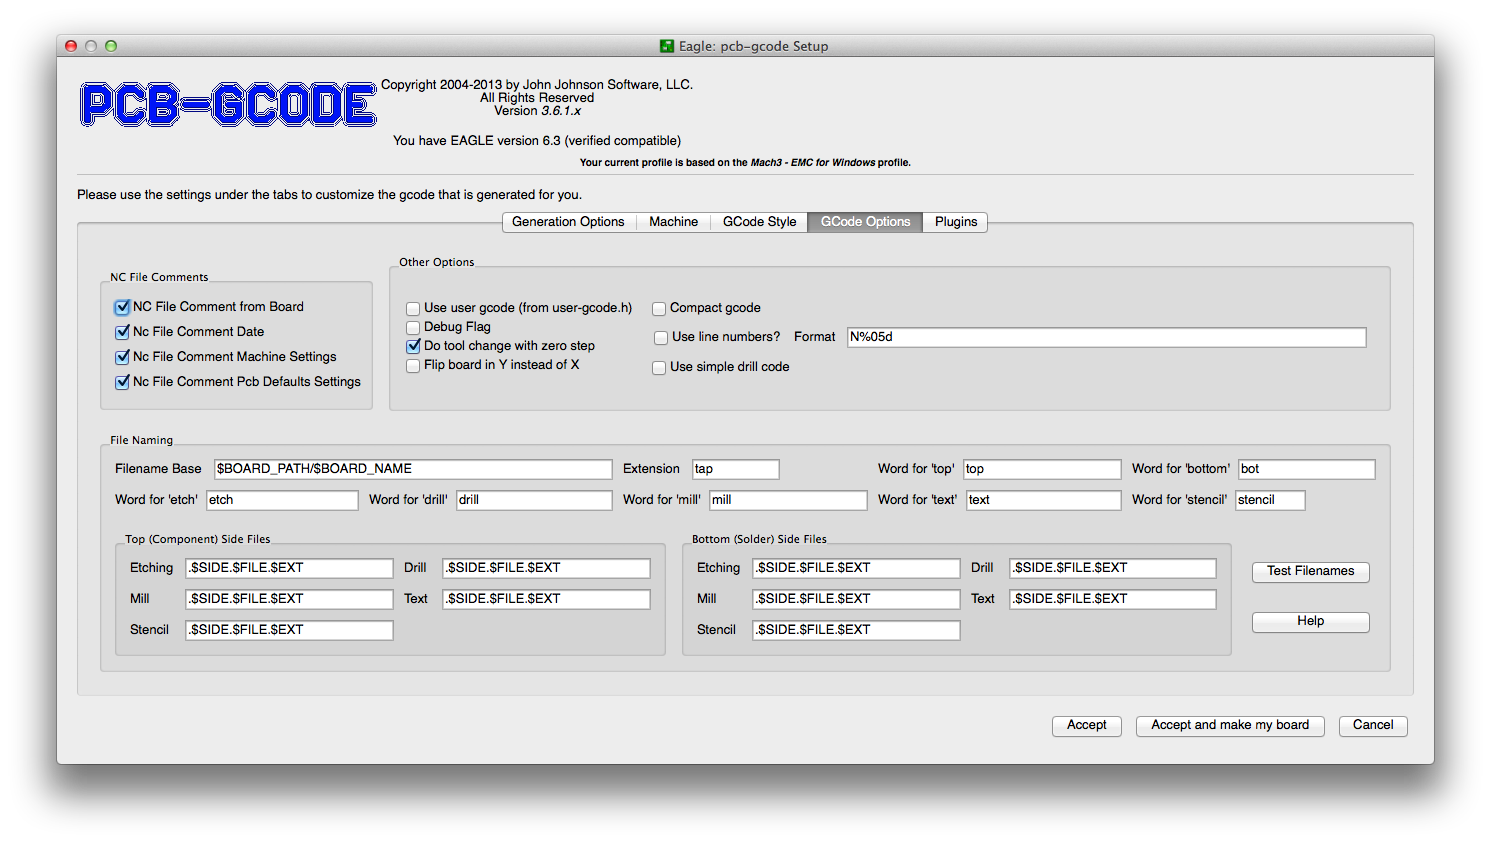
\includegraphics[width=14cm]{figs/Setup-GCode-Options.png}
	}
	\caption{Options for generating g-code files.}
	\label{fig:GCodeOptions}
\end{figure}\index{setup tabs!GCode Options}

The options under the GCode Options tab allows the customization of some of the g-code file's content, as well as how the files are named.

\begin{description}
	\item[NC File Comments] Comments added to the g-code file.\index{g-code!comments}
	\begin{description}
		\item[NC File Comment from Board] adds a comment with the name of the board file.
		\item[NC File Comment Date] adds the date the g-code file is created.
		\item[NC File Comment Machine Settings] adds settings related to the machine. Tool size, Z axis settings, spindle on time, milling depth, text depth, tool change position, XY feed rate, Z feed rate.
		\item[NC File Comment PCB Defaults Settings] adds comments with the isolation settings: min, max, and step size, which files were selected to be produced, and the unit of measure.
	\end{description}
	
	\item[Other Options] Options affecting how the g-code is generated.
	\begin{description}
		\item[Use user gcode (from user-gcode.h)] inserts user g-code into the generated file. See Section \vref{sec:UserGCode} for more details.\index{g-code!user}
		\item[Debug Flag] sets the global debug flag. Used for development and troubleshooting.
		\item[Do tool change with zero step] after moving to the tool change position and pausing for the operator to change the bit, the Z axis will move to Z0.000 and pause. This allows the operator to adjust the bit length to touch the surface of the PCB. Note that the tool should initially be set high into the spindle so that it won't dig into the PCB when it moves to Z0.\index{tool change!zero step}
		\item[Flip board in Y instead of X] changes the code generated so that after one side of the board is cut, the board should be flipped in the Y axis to complete cutting on the other side. The default is for the board to be flipped in the X axis.
		\item[Compact gcode] eliminates some redundant commands in the g-code file, such as having G01 on every line.\index{g-code!compact}
		\item[Use line numbers?] inserts line numbers into the g-code file. The format shown \code{\%05d} will insert 5 digit numbers with leading zeroes.\index{g-code!line numbers}
		\item[Use simple drill code] uses simple XYZ movements to create drill holes. Usually \code{DRILL\_{}FIRST\_{}HOLE} and \code{DRILL\_{}HOLE} are used, but some controllers don't understand the command (typically \code{G82}).\index{drill!simple g-code}
	\end{description}
	
	\item[File naming] every option one could want for naming files.\index{files!naming}
	\begin{description}
		\item[Macros] the following can be used in the file name to create the final file name. Note that paths do not include a \code{/} at the end. Also note that \code{/} is always the path delimiter, even on Windows. Eagle handles the conversion automatically.
		\begin{description}
			\item[\$PROJECT\_{}PATH{[}n{]}] Project paths as set in the Eagle Control Panel. n begins at zero for the first entry.
			\item[\$ULP\_{}PATH{[}n{]}] ULP paths as set in the Control Panel.
			\item[\$CAM\_{}PATH{[}n{]}] CAM paths as set in the Control Panel.
			\item[\$BOARD\_{}PATH] path to the board file.
			\item[\$BOARD\_{}NAME] the file name of the board file with the extension removed.
			\item[\$SIDE] the side of the board being generated. Defaults are 'bot' and 'top'.
			\item[\$FILE] the file being generated. Defaults are 'etch', 'drill', 'mill' and 'text'.
			\item[\$EXT] the extension set in \code{Extension} on this screen.
		\end{description}
		\item[Test Filenames] click the button to see how the file names will look.
		\item[Help] gives a list of the macros defined above and tips on creating file names.
	\end{description}
\end{description}

Using the options shown in \ref{fig:GCodeOptions}, here is how the filename for the top etching file will be created:
\begin{itemize}
\item The board path and board name will be used. (\code{Filename Base})
\item The word for 'top' will be substituted for \code{\$SIDE}. (See \code{Etching} under \code{Top (Component) Side Files}.
\item The word for 'etch' will be substituted for \code{\$FILE}.
\item The \code{Extension} will be substituted for \code{\$EXT}.
\end{itemize}
Using examples for the board path and name, the final file name would be:\\
\lstinline!/Users/john/Documents/pcbcode/examples/enabtmr.top.etch.tap!

%
%---------------------------------------------------------------------
%
\newpage
\section{Support}\label{sec:Support}\index{support}

Several options are available for support. First and foremost, read this manual and ensure that your question is not herein.

\begin{description}
    \item[Yahoo! Group] The \href{https://groups.yahoo.com/group/pcb-gcode}{Yahoo! group} has over 3 000 members, many of whom are very active and experienced in the use of pcb-gcode.\index{support!Yahoo group}
    \item[Phorum] The \href{http://pcbgcode.org}{online BBS} where questions and answers may be posted, files downloaded, etc.\index{support!Phorum}
    \item[Email] Very limited \href{mailto:pcbgcode@pcbgcode.org}{email support} is available. Please try all the other options first.
    \item[On\-site Support] If you are in the Atlanta area, on\-site support is a possibility. Please \href{mailto:pcbgcode@pcbgcode.org}{email me}.\index{support!on site}
\end{description}


%======================================================================
%
\chapter{Using pcb-gcode}
%
%======================================================================

%
%---------------------------------------------------------------------
%
\section{Running pcb-gcode}\index{pcb-gcode!running}\label{sec:running}

Run pcb-gcode by selecting File $|$ Run... from EAGLE's board editor. Find the file \code{pcb-gcode-setup.ulp} and click the Open button. The setup screen will be shown where options can be changed (See \figurename~\ref{fig:SetupGenerationOptions}). When the options are correct, click the \code{Accept and make my board} button. To save the options without generating files for the board, click the \code{Accept} button.

Pcb-gcode is actually two programs. The first, \code{pcb-gcode-setup}, allows for setting options and changing the way NC files are created. The second program is \code{pcb-gcode}, which actually creates the files. Most people run \code{pcb-gcode-setup}, check their settings, then click the \code{Accept and make my board} button to generate files. If settings don't need to be changed, \code{pcb-gcode} can be run directly and all the file selections and options from the last time \code{pcb-gcode-setup} was run will be used.

To make it easier to run \code{pcb-gcode} and \code{pcb-gcode-setup}, use EAGLE's Assign function to assign a shortcut key to \code{run pcb-gcode} and \code{run pcb-gcode-setup} (See \figurename~\vref{fig:EagleOptionsAssign}).

\begin{figure}
	\center{
	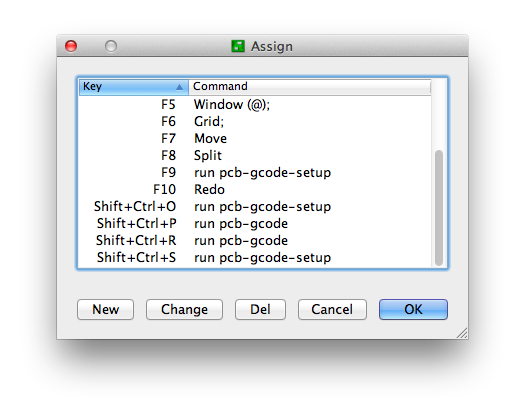
\includegraphics[width=5cm]{figs/EAGLE-Options-Assign.png}
	}
	\caption{EAGLE shortcut key assignments.}
	\label{fig:EagleOptionsAssign}
\end{figure}

%
%---------------------------------------------------------------------
%
\section{Using EAGLE's DRC}\index{eagle!DRC}\label{sec:EagleDRC}

When creating files to etch a board, it is usually the case that the tracks should be made wide to allow for easier machining and to account for tolerances in the machine such as backlash and spindle runout. EAGLE's Design Rule Check (DRC) can be used to help ensure that all tracks on the board will be cut out, and no bridges will be left. 

A bridge is formed when two parts (tracks, pads, vias) on the board are too close together for the etching tool to pass between them.\index{bridges} An example is shown in \figurename~\vref{fig:TwoComponents}. For this example, Single Pass isolation is selected, minimum isolation is set to $0.010''$, and the etching tool size is set to $0.005''$. These setting are shown in \figurename~\vref{fig:DRCExampleSettings}.

\begin{figure}
	\center{
	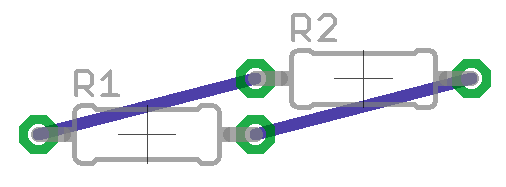
\includegraphics[width=5cm]{figs/Two-Components.png}
	}
	\caption{Two components in the board layout editor.}
	\label{fig:TwoComponents}
\end{figure}

\begin{figure}
	\center{
	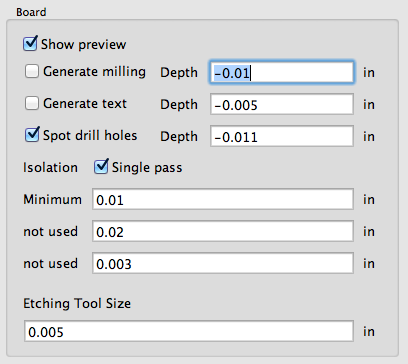
\includegraphics[width=5cm]{figs/DRC-Example-Settings.png}
	}
	\caption{Pcb-gcode settings for the DRC example.}
	\label{fig:DRCExampleSettings}
\end{figure}

If the pads for the leads for the resistors that are close together are more than $0.010'' + 0.010'' + 0.005'' = 0.025''$ inches apart, the pads will be properly isolated as shown in \figurename~\vref{fig:GoodClearance}. However, if the two pads are less than $0.025''$ apart, they cannot be isolated, and a bridge will be formed as shown in \figurename~\vref{fig:TooClose}.

\begin{figure}
	\center{
	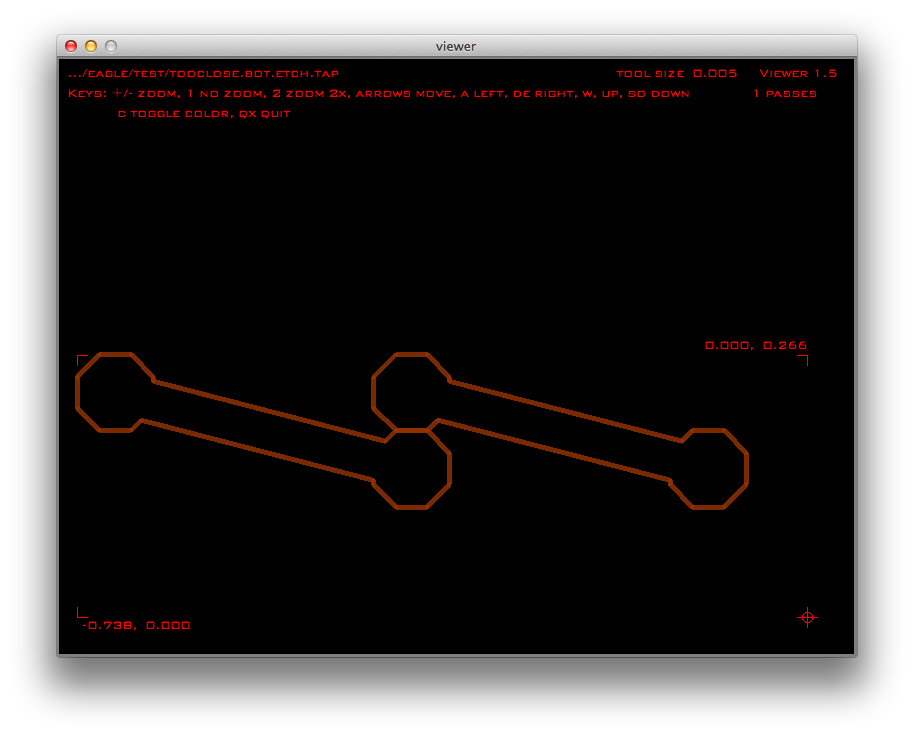
\includegraphics[width=7cm]{figs/Good-Clearance.png}
	}
	\caption{The pads are far enough apart to allow them to be isolated.}
	\label{fig:GoodClearance}
\end{figure}

\begin{figure}
	\center{
	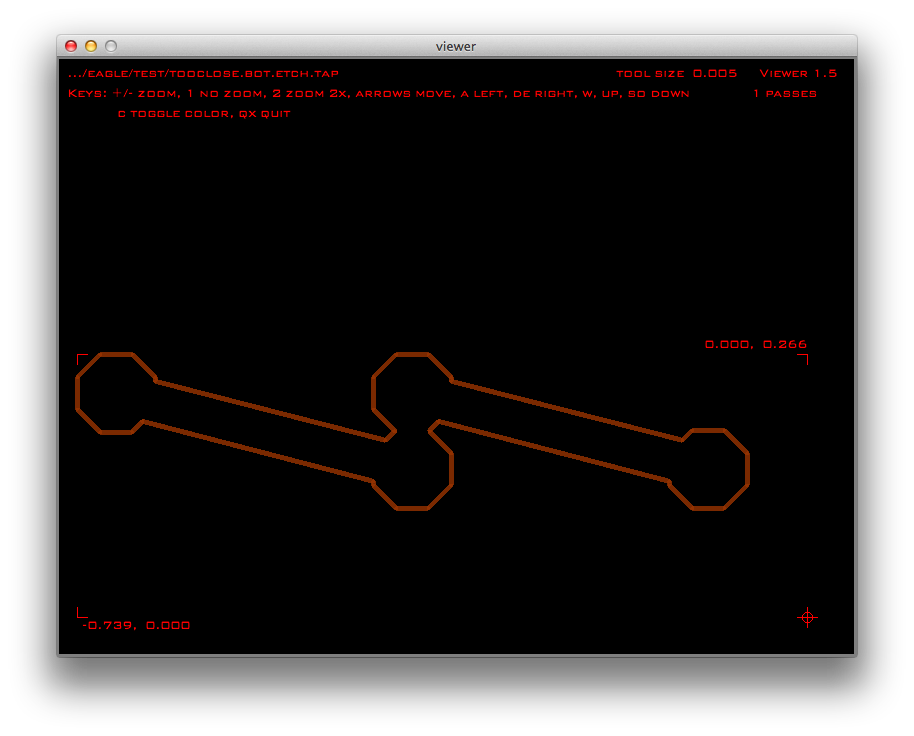
\includegraphics[width=7cm]{figs/Too-Close.png}
	}
	\caption{The two pads are too close together and cannot be isolated. A bridge is formed.}
	\label{fig:TooClose}
\end{figure}

To help ensure that this does not happen, EAGLE's DRC can be used. From the board editor in EAGLE, click the Tools menu, then click DRC. Click the Clearance tab and set all clearances to 25mil. (A mil is $0.001''$, so this equals $0.025''$.) When the Check button is clicked, any distances less than 0.025" will be marked with a red mark, and a list of errors will be shown as in \figurename~\vref{fig:DRCError}.

\begin{figure}
	\center{
	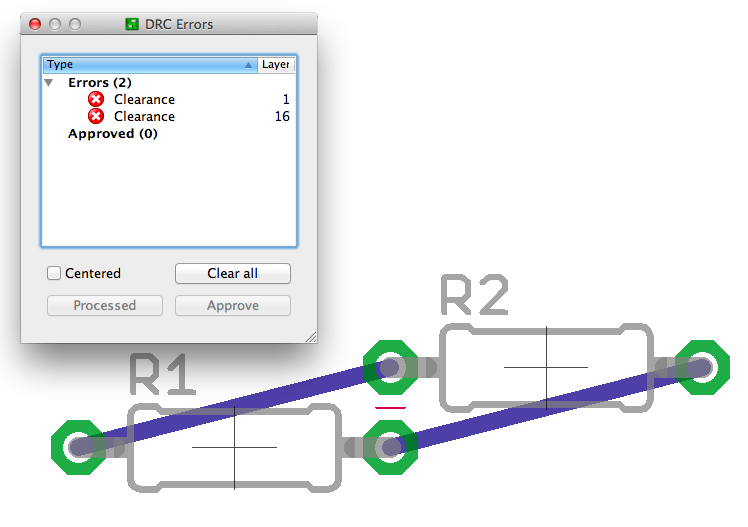
\includegraphics[width=7cm]{figs/DRC-Error.png}
	}
	\caption{EAGLE's DRC indicating the two pads are too close together.}
	\label{fig:DRCError}
\end{figure}

Once the DRC clearances are set up, it is a simple matter to click the DRC button or run a DRC check from the Tools menu before running pcb-gcode to generate files for the board. This provides a good way to help ensure that components on the board are far enough apart to be properly isolated.

%
%---------------------------------------------------------------------
%
\section{Previewer}\index{previewer}\label{sec:Previewer}

The previewer included in pcb-gcode shows a quick preview of the tool movements that are sent to the NC file. The lines are color coded using the standard resistor color codes. The first pass of the tool is drawn in brown, the second is red, the third is orange, etc.

The preview is enabled by turning on the \code{Show preview} option under the \code{Generation Options} tab (See \figurename \vref{fig:SetupGenerationOptions}). After pcb-gcode creates the isolation or milling for the current layer, a preview of the results will be shown in the previewer. Several keys can be used to change the view, See Table \vref{tbl:PreviewerKeys}. If you wonder about some of the unusual keys, such as why \code{e} can be used to pan right, it is because of the Dvorak keyboard layout that some use, including the author.

\begin{table}[h]\caption{Keys available in previewer}\label{tbl:PreviewerKeys}\index{previewer!keys}\index{keys!previewer}
\centering
\begin{tabular}{ll}
	\toprule
	Key 		& Function\\ 
	\midrule
	1		& Set zoom to 1x (no zoom)\\
	2		& Set zoom to 2x\\
	+ =		& Zoom in\\
	- \_{}		& Zoom out\\
	a $\leftarrow$ & Pan left\\
	d e $\rightarrow$ & Pan right\\
	w , $\uparrow$ & Pan up\\
	s o $\downarrow$ & Pan down\\
	c		& Color on / off\\
	q x		& Quit preview \\ \bottomrule
\end{tabular}
\end{table}

The previewer does not read and interpret the NC files directly, but uses an internal representation of the tool movements. This gives an accurate representation of the tool's movements and size, without the overhead of interpreting several different styles of g-code.

\begin{figure}
	\center{
	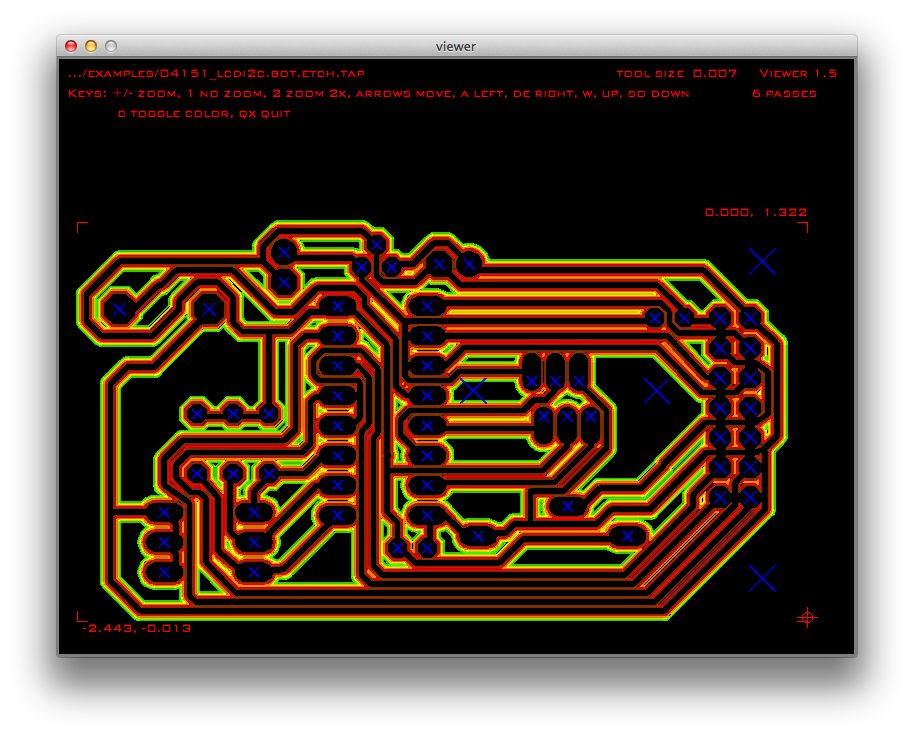
\includegraphics[width=14cm]{figs/Previewer-Screen-Shot.png}
	}
	\caption{The previewer showing a multi-pass file for the bottom side of an example PCB included with pcb-gcode. Each $\times$ represents a drill hole in the drill file.}
	\label{fig:PreviewerScreenShot}
\end{figure}

As can be seen in \figurename~\vref{fig:PreviewerScreenShot}, additional information is provided by the preview. In the upper-left corner is the name of the board file that was processed to produce this preview. At the upper-right, the viewer version number can be found. Just to the left of that is the etching tool size set in pcb-gcode-setup. Just below the version number is the number of passes generated. Back on the left-hand side near the top is an overview of the keys available.

The four extents of the board are marked with red corners. At the upper right corner, the X and Y coordinates are given. The X and Y coordinates are also given at the lower-left corner. Note that in the figure, the X coordinate is negative because this is the bottom of the board. In the lower right corner, a circle and crosshairs mark the origin point for the board.

If the milling and text options are turned on, the previewer will show any files generated for the top and bottom milling and text. Since the Milling (46) layer is not a top or bottom layer (it can be thought of as going through the board), NC files are generated to mill any lines drawn on it from either the top or bottom side. So in other words, if \code{Generate milling} is selected, both top and bottom milling files will be generated. The same for text placed on the Milling layer. If \code{Generate text} is selected, both top and bottom text engraving files will be generated. There is one caveat: if the text is mirrored, it will be output in the bottom milling file. If the text is not mirrored, it will be output in the top milling file. This is similar to the way text placed on the \code{Top} and \code{Bottom} layers looks. The following example will help clarify this.

The example board \code{docs/examples/04151\_lcdi2c.brd} shown in \figurename~\vref{fig:014151Board} includes wires (shown in blue) drawn on the Milling layer, as well as mirrored vector text (also shown in blue) placed on the Milling layer. A prewiew of the bottom milling file is shown in \figurename~\vref{fig:BottomMilling}. A preview of the bottom text engraving file is shown in \figurename~\vref{fig:BottomText}. You can see that the text is oriented properly for engraving on the bottom side of the board. The object info for the text is shown in \figurename~\vref{fig:MirroredTextInfo}.

The top milling file preview looks just like the bottom preview, and is not shown. The top text engraving file was empty since there is no non-mirrored text on the Milling layer, so its preview has also been omitted.

\begin{figure}
	\center{
	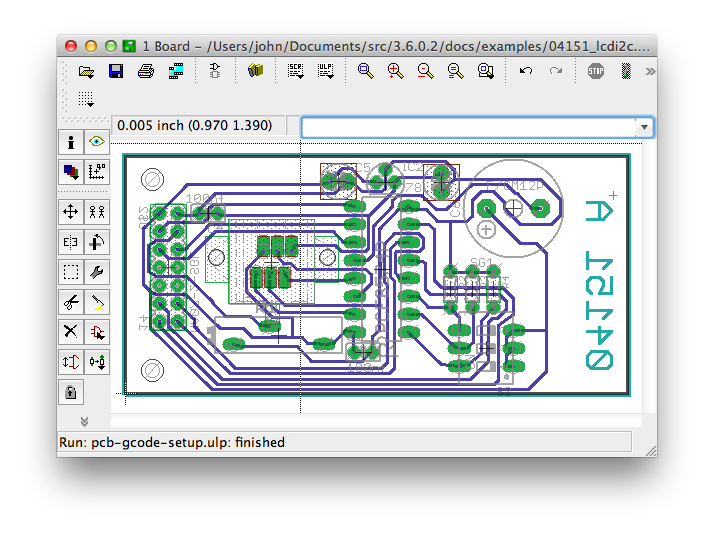
\includegraphics[width=10cm]{figs/04151_lcdi2c.png}
	}
	\caption{The sample board \code{docs/examples/04151\_lcdi2c.brd} with wires and mirrored text on the Milling layer.}
	\label{fig:014151Board}
\end{figure}

\begin{figure}
	\center{
	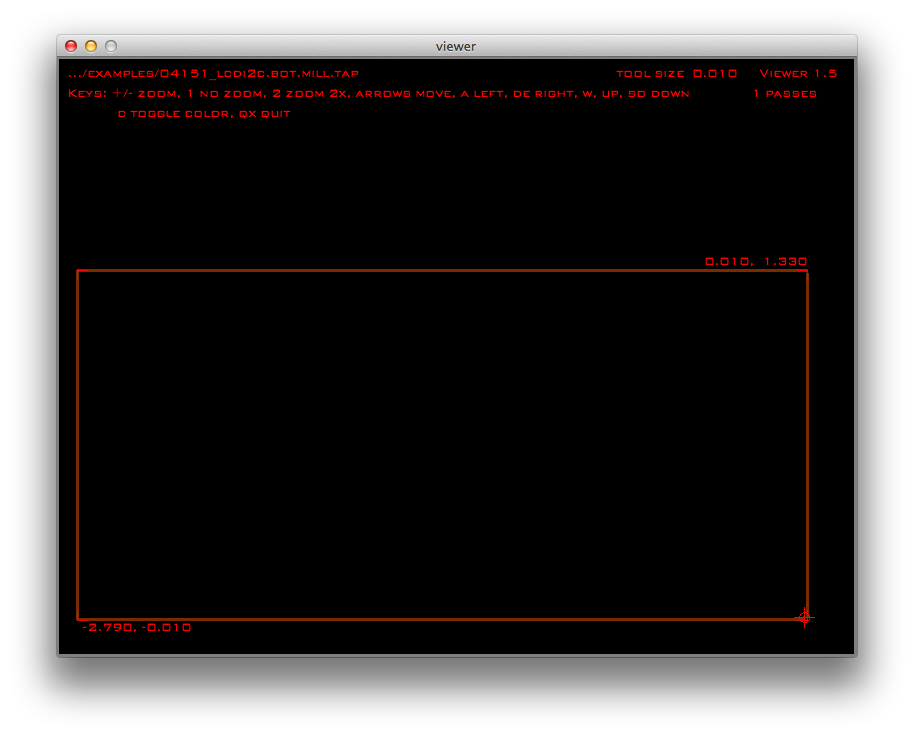
\includegraphics[width=10cm]{figs/Bottom-Milling.png}
	}
	\caption{Milling generated for milling from the bottom side of \code{docs/examples/04151\_lcdi2c.brd}.}
	\label{fig:BottomMilling}
\end{figure}

\begin{figure}
	\center{
	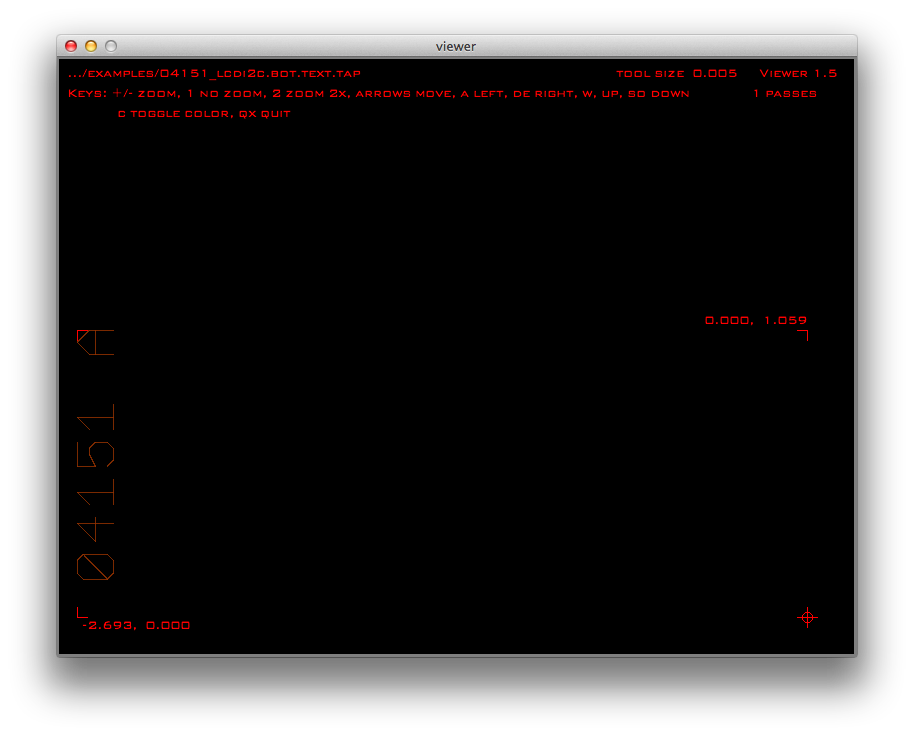
\includegraphics[width=10cm]{figs/Bottom-Text.png}
	}
	\caption{Text engraving generated for cutting on the bottom side of \code{docs/examples/04151\_lcdi2c.brd}.}
	\label{fig:BottomText}
\end{figure}

\clearpage

\begin{figure}
	\center{
	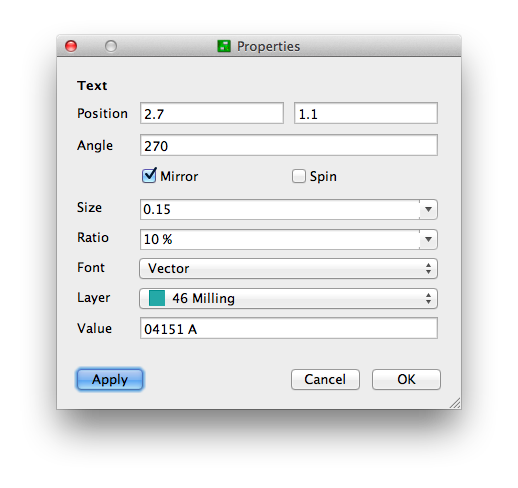
\includegraphics[width=8cm]{figs/Mirrored-Text-Info.png}
	}
	\caption{The object info for the mirrored text on the Milling layer. Note that the Mirror checkbox is on. This indicates to pcb-gcode that the text should be engraved on the bottom side of the board.}
	\label{fig:MirroredTextInfo}
\end{figure}


\howitworks{}
For the curious reader, the previewer is written using a language called \href{http://processing.org}{Processing}, which is somewhat Java-like. Three versions of the previewer are included in pcb-gcode, one for each operating system supported: Mac OS X, Linux, and Windows. When the previewer is enabled, pcb-gcode detects which operating system it is running on, and runs the appropriate viewer.

%
%---------------------------------------------------------------------
%
\section{Saving and Loading Settings}\label{sec:SaveSettings}

\subsection{Overview}\index{settings!saving and loading}

\begin{figure}
	\center{
	\includegraphics[width=16cm]{figs/Setup-PlugIns.png}
	}
	\caption{The Plugins tab showing where settings can be saved and loaded.}
	\label{fig:SaveSettings}
\end{figure}\index{setup tabs!Plugins}

Settings may be loaded and saved to settings files. This can be found on the Plugins tab, and is shown in figure \vref{fig:SaveSettings}. This allows the operator to set up groups of settings for different PC boards, save them, and load them when manufacturing the same board later. The settings saved include those on the Generation Options tab (shown in figure \vref{fig:SetupGenerationOptions}), as well as those on the Machine tab (see figure \vref{fig:SetupMachine}) except for the Units setting.

\subsection{Saving Settings}\index{settings!saving}

First, set up all settings on the Generation Options tab, and the Machine tab. When the settings are working as desired, select the Plugins tab, then click the \code{Save as} button. A standard file save dialog will appear where you can enter a file name. A confirmation dialog will appear telling you your settings have been saved, then setup will reload.

If you would like to replace a set of settings that have already been saved, click the filename in the list of Settings, then click the Save button. A dialog will open confirming that your settings have been saved.
\\

\warning{Eagle Bug}
\textbf{Note that settings must be saved in the \code{<pcb-gcode path>/settings/saved} folder.}\index{settings!path to}
There is a bug on some platforms that prevents pcb-gcode from setting the proper directory for the save dialog. Please ensure the directory is set correctly, otherwise your saved files will not appear in the list of Settings.
\\

\subsection{Loading Settings}\index{settings!loading}

To load a set of settings you have saved before, go to the Plugins tab, select the file from the Settings list, and click the Load button. The settings will be loaded, and the setup program will reload.

\information{Intermediate}
The settings from the Generation Options tab are saved in \code{pcb-defaults.h}, and the settings from the Machine tab are saved in \code{pcb-machine.h}. When the settings are saved from the Plugins tab, they are copied to \code{filename.def} and \code{filename.mac} files. When loading, the opposite operation takes place.

%======================================================================
%
\chapter{Customizing}
%
%======================================================================

%
%---------------------------------------------------------------------
%
\section{G-Code}\index{g-code!customizing}\label{sec:CustomizingGCode}

\warning{Intermediate}
When the g-code style is initially selected at installation as discussed in Section \vref{sub:SelectingGCodeStyle}, the profile (\code{.pp}) file selected is copied from the \code{profiles} folder to the \code{settings} folder and to the file \code{gcode-defaults.h}. This is the file that pcb-gcode uses when generating g-code files.

The listing found in Appendix \vref{chp:SampleProfile} can alse be used as a reference for editing \code{gcode-defaults.h}. If there is a need to change the g-code generated by pcb-gcode, the gcode-defaults.h file can be edited.

The definitions in the file are flexible in some aspects, and restricted in others. The main restriction is that a definition that expects a certain number of parameters must be given that number of parameters. Unused parameters can be passed as comments in the g-code. 

For example, if the controller does not understand the DWELL command, it can be changed to a comment. In the listing, DWELL is defined to be:

\begin{lstlisting}[firstnumber=46]
string DWELL   = "G04 " + PARAM + "%f" + EOL;
\end{lstlisting}

This can be made into a comment the controller will ignore by surrounding it with COMMENT\_{}BEGIN and COMMENT\_{}END:

\begin{lstlisting}[firstnumber=46]
string DWELL   = COMMENT_BEGIN + "G04 " + PARAM + "%f" + COMMENT_END + EOL;
\end{lstlisting}

The \lstinline!%f! that pcb-gcode needs is still there, but the command is now just a comment as far as the controller is concerned.

\marginpar{\scriptsize This is only an example. EAGLE handles line endings automatically depending on the operating system it is running on. If line endings in generated NC files need to be changed, a conversion program should be used.}

The definitions use previous definitions as much as possible. This helps make the files more readable, and makes future changes easier as well. For instance, \code{EOL} is defined in line 22 to be \code{"\textbackslash{}n"}. Changing the line ending of all generated code would be a simple matter of changing the single definition of \code{EOL}, rather than editing every line.

The first option on line 11, \code{FILENAMES\_8\_CHARACTERS}, tells pcb-gcode whether it should limit filenames to 8 characters. This is used for DOS control software such as TurboCNC.

\begin{description}\index{gcode-defaults.h!definitions of commands}\index{profiles!definitions of commands}
\item[Misc defines] Comments and line ending
\begin{description}
	\item[COMMENT\_{}BEGIN, COMMENT\_{}END] If your controller doesn't understand beginning and ending characters for comments, as on lines 16-17, just make \code{COMMENT\_{}END} empty.

	\item[EOL] is the character added to the end of every line.
\end{description}

\item[Formats] Parameter formats.
\begin{description}
    \item[PARAM] different controllers use different characters to introduce a parameter. Mach3 uses \code{P}, while others use \code{\#}.
    
    \item[FORMAT] is the floating point format used for coordinates. The default value \code{\%-7.4f} means a leading negative sign will be output for negative coordinates (very important), the number will be 7 digits long, and 4 digits will be to the right of the decimal point. The \code{f} indicates it is a floating point (real) number.
    
    \item[FR\_{}FORMAT] is the format used to insert feedrate parameters into the g-code. In the example, the leading \code{F} indicates this is a feedrate parameter. The rest of the format is similar to \code{FORMAT} --- leading negative sign possible, 5 digits wide, no digits to the right of the decimal point.
    
    \item[IJ\_{}FORMAT] is used to output \code{I J} coordinates to the g-code file. You can see by the definition on line 26 that this format reuses the \code{FORMAT} definition defined earlier.
    
    \item[R\_{}FORMAT] is used by commands that require an \code{R} parameter, usually the radius for an arc command.
\end{description}

\item[Modes] Inch, metric, etc. modes
\begin{description}
    \item[INCH\_{}MODE] used to set the controller to inch mode.
    
    \item[INCH\_{}MODE\_{}COMMENT] a comment inserted in the g-code indicating that inch mode is being set.
    
    \item[METRIC\_{}MODE] used to set the controller to Metric mode.
    
    \item[METRIC|\_{}MODE\_{}COMMENT] a comment inserted in the g-code indicating that metric mode is being set.
    
    \item[MIL\_{}MODE] used to set the controller to mil mode. Currently undefined in all profiles.
    
    \item[MICRON\_{}MODE] used to set the controller to micron mode. Currently undefined in all profiles.
    
    \item[ABSOLUTE\_{}MODE] would be used to set the controller to absolute coordinates mode. Currently just a comment.
\end{description}

\item[G Codes] Basic g-code defines for movements.
\begin{description}
    \item[RAPID] for rapid moves with the cutting tool out of the material.
    \item[FEED] for movements with the cutting tool in the material.
    \item[ARC\_{}CW] for cutting an arc clockwise.
    \item[ARC\_{}CCW] for cutting an arc counter-clockwise.
    \item[DWELL] pause for a number of seconds. Number of seconds (a float) is passed.
\end{description}

\item[M Codes] M-code definitions.
\begin{description}
	\item[SPINDLE\_{}ON] turns the spindle on. Takes \code{DWELL} as a parameter.
	\item[SPINDLE\_{}OFF] turns the spindle off.
	\item[END\_{}PROGRAM] signals the end of the gcode program.
	\item[OPERATOR\_{}PAUSE] pauses for the operator to do something, like change the tool.
\end{description}

\item[Coordinates] Definitions for coordinate parameters.
\begin{description}
	\item[MOVE\_{}X] X axis movement. Passed an \code{X} coordinate as a parameter.
	\item[MOVE\_{}Y] Y axis movement. Passed a \code{Y} coordinate as a parameter.
	\item[MOVE\_{}XY] XY axis movement. Passed an \code{X} and \code{Y} coordinate as parameters.
	\item[MOVE\_{}Z] Z axis movement. Passed a \code{Z} coordinate as a parameter.
	\item[MOVE\_{}XYZ] XYZ axis movement. Passed \code{X Y Z} coordinates as parameters.
\end{description}

\item[Rapids] Combinations of \code{RAPID} and the above coordinates.
\begin{description}
	\item[RAPID\_{}MOVE\_{}X] rapid X axis movement. Passed an \code{X} coordinate as a parameter.
	\item[RAPID\_{}MOVE\_{}Y] rapid Y axis movement. Passed a \code{Y} coordinate as a parameter.
	\item[RAPID\_{}MOVE\_{}XY] rapid XY axis movement. Passed \code{X Y} coordinates as parameters.
	\item[RAPID\_{}MOVE\_{}XY\_{}HOME] rapid XY axis movement to \code{X0 Y0}.
	\item[RAPID\_{}MOVE\_{}Z] rapid Z axis movement. Passed a \code{Z} coordinate as a parameter.
	\item[RAPID\_{}MOVE\_{}XYZ] rapid XYZ axis movement. Passed \code{X Y Z} coordinates as parameters.
\end{description}

\item[Feeds] Movements at cutting speed, uses \code{FEED} and the coordinate definitions above.
\begin{description}
	\item[FEED\_{}MOVE\_{}X] feed X axis movement. Passed an \code{X} coordinate as a parameter.
	\item[FEED\_{}MOVE\_{}Y] feed Y axis movement. Passed a \code{Y} coordinate as a parameter.
	\item[FEED\_{}MOVE\_{}XY] feed XY axis movement. Passed \code{X Y} coordinates as parameters.
	\item[FEED\_{}MOVE\_{}XY\_{}WITH\_{}RATE] feed XY axis movement. Passed \code{X Y} coordinates and the feed rate.
	\item[FEED\_{}MOVE\_{}Z] feed Z axis movement. Passed a \code{Z} coordinate as a parameter.
	\item[FEED\_{}MOVE\_{}Z\_{}WITH\_{}RATE] feed Z axis movement. Passed \code{Z} coordinate and a feed rate as parameters.
	\item[FEED\_{}MOVE\_{}XYZ] feed XYZ axis movement. Passed an \code{X Y Z} coordinates as parameters.
\end{description}

\item[Drilling holes] Definitions for drilling holes.
\begin{description}
	\item[DRILL\_{}CODE] the gcode instruction to drill a hole.
	\item[RELEASE\_{}PLANE] the Z position to move the drill to after drilling. Takes a \code{Z} coordinate as a parameter.
	\item[DWELL\_{}TIME] the time to dwell in the bottom of the hole. Takes a floating point (real) argument.
	\item[DRILL\_{}FIRST\_{}HOLE] generated to drill the first hole. Takes \code{X Y Z}, feed rate, release \code{Z} plane and dwell time as parameters.
	\item[DRILL\_{}HOLE] generated for subsequent holes. Takes \code{X Y} as parameters.
\end{description}

\item[Tool change] Definitions for changing tools.
\begin{description}
	\item[TOOL\_{}CODE] the tool selection code. Passed the tool number (an integer) as a parameter.
	\item[TOOL\_{}MM\_{}FORMAT] a tool size formatted for millimeters. Passed a tool size (float).
	\item[TOOL\_{}INCH\_{}FORMAT] a tool size formatted for inches. Passed a tool size (float).
	\item[TOOL\_{}CHANGE] the command issued when a tool is to be changed. Takes tool number and tool size as arguments.
	\item[TOOL\_{}CHANGE\_{}TABLE\_{}HEADER] the tool table header comment inserted in the g-code.
	\item[TOOL\_{}CHANGE\_{}TABLE\_{}FORMAT] generates an entry for the tool table. Note that this is a function.
\end{description}

\item[Circles / Arcs] Arc and circle commands.
\begin{description}
	\item[ARC\_{}TOP] is an arc on the top of the board. Takes \code{X Y R} as parameters.
	\item[ARC\_{}BOTTOM] an arc on the bottom of the board. Takes \code{X Y R} as parameters.
\end{description}
\end{description}

%
%---------------------------------------------------------------------
%
\section{Profiles}\index{profiles}\label{sec:Profiles}\index{g-code!profiles}

\warning{Advanced}
Profiles, which are found in the \code{profiles} folder, control the format that pcb-gcode uses when writing g-code. The files ending in \code{.pp} are the list of files shown when pcb-gcode is initially set up (See Section \vref{sec:Installation}), and also in the list of profiles in the \code{GCode Styles} tab. When a profile is selected, it is copied to \code{settings/gcode-defaults.h}. A sample profile is shown in Appendix \vref{chp:SampleProfile}. 

To create a custom profile, such as for a controller that is not already supported, begin with a profile that most closely matches the g-code the controller supports. Select this profile in \code{GCode Styles} and \code{Accept} the change. This will copy the profile to \code{settings/gcode-defaults.h}. Generate code for a test board and open the generated files in an editor. Find commands that the controller does not support, and edit \code{gcode-defaults.h} to generate the proper code. When testing is complete, copy \code{settings/gcode-defaults.h} into the \code{profiles} folder, renaming it with a descriptive name and the extension \code{.pp}. Edit the file and change the author and description fields. And of course, save a backup somewhere outside the pcb-gcode folder heirarchy. To share this profile with other users of this controller, upload the profile file to the \href{http://groups.yahoo.com/group/pcb-gcode/files/%21%20Software/Profiles/}{Profiles folder} on the Yahoo! group.

For information on editing \code{gcode-defaults.h}, See Section \vref{sec:CustomizingGCode}.


%
%---------------------------------------------------------------------
%
\section{Drill Rack Files}\index{drill!rack files}\index{drill!substitutions}\label{sec:DrillRackFiles}

Rack files allow the substitution of one drill size for a range of sizes that may be found in the board. For instance, a $0.031''$ drill might be used for hole sizes $0.025''$ -- $0.032''$. This cuts down on the number of drills that must be kept on hand, and the number of tool changes needed to drill a board. An example drill rack file is shown in Listing \ref{lst:SampleRackFile}. \textbf{Please heed the warning about using a tab character} between entries on a line. Otherwise, your rack file will not work.

As can be seen, drills with different units of measure are supported. This includes inches, millimeters, mils, or wire gage sizes. See Listing \ref{lst:SampleEntries} for examples that work. The algorithm tries to be intelligent and assumes, for example, that 0.1 is in inches, whereas 0.6 is in millimeters. To be safe, add the unit of measure after the number.

Looking at Listing \ref{lst:SampleRackFile}, the meaning of the fields are as follows:

\begin{description}
	\item[tool] The tool number to use. This is somewhat arbitrary unless the machine has a tool changer or you have offsets or lengths set up for different tool numbers. Tool numbers can begin at any reasonable number, such as T01, T16, etc.
	\item[drill\_size] The size of the actual drill. These should be in ascending order from smallest to largest.
	\item[minimum] The smallest hole size this drill should be used for.
	\item[maximum] The largest hole this drill should be used for.
	\item[length] Currently not used. Leave set to 1.5in.
\end{description}

Taking tool \code{T01} as an example. It is a 0.500mm drill, and it will be used for all holes from \code{0.000in} up to \code{0.025in}. Meaning, if there is a $0.015''$ hole in the board, it will be drilled with this bit. If there is a $0.045''$ hole, it will not be drilled with drill \code{T01}, but another drill will be used, if a good match is available.

Looking at the table, it can be seen that all hole sizes from 0.000in up to 0.125in have been accounted for. If, say, a $0.130''$ hole is in the board, an error message will be given saying a drill is not available for that size hole.

Rack file are selected by the following method: first, if there is a rack file with the same name as the board, but with the extension \code{.drl}, it will be used. Next, a default rack file will be used if it has been set in \code{pcb-gcode-setup} (See \figurename \vref{fig:SetupMachine}). Finally, if neither of those is available, the rack file \code{settings/default.drl} will be used from the \code{pcb-gcode} directory. If all these attempts fail and no rack file can be found, a table of drill sizes will be written to the drill file. In most cases this works well, but sometimes it can result in, for instance, drilling ten holes with a $0.031''$, then stopping and asking for a $0.032''$ bit. Obviously, the same bit could have been used for both sets of holes. That is why rack files exist.


\begin{lstlisting}[caption={Sample Rack File},label={lst:SampleRackFile}]
#
# Please note that you must use a TAB character
# between each setting on a line.
# 
# Tip: Set the TAB size of your editor to 12 characters.
#
tool	drill_size	minimum	maximum	length
T01	0.500mm		0.000in	0.025in	1.5in
T02	0.032in		0.025in	0.035in	1.5in
T03	0.040in		0.035in	0.045in	1.5in
T04	0.050in		0.045in	0.055in	1.5in
T05	0.062in		0.055in	0.070in	1.5in
T06	0.085in		0.070in	0.125in	1.5in
\end{lstlisting}

\begin{nbcode}[caption={Sample entries for rack files},label={lst:SampleEntries}]
0.032in   0.032 inches
62ml      62 mils, 0.062 inches
0.43mm    0.43 millimeters
1500mc    1500 microns, 1.500 millimeters
60#       60 wire gage drill (0.040'' or 1.016mm)
0.12      0.12 inches
0.60      0.60 millimeters
43        43 wire gage drill
\end{nbcode}



%
%---------------------------------------------------------------------
%
\section{User GCode}\index{user gcode}\label{sec:UserGCode}\index{g-code!user}

\warning{Advanced}
The pcb-gcode ULP allows you to customize the g-code created for your boards to a great degree. If you don't see an option in the profile that suits your needs, you can add your code to the \code{user-gcode.h} file. To enable user g-code, run \code{pcb-gcode-setup}, click the \code{GCode Options} tab, then turn the \code{Use user gcode...} option on. Generate a set of NC files for a board. Let's say, for example, that after you change the tool when you're drilling from the bottom of the board, you want the tool to move to X5 Y5 Z5, turn the spindle off, then turn it back on. Since this has to do with drilling the bottom of the board, we should look at the ...bot.drill.tap (bottom drill) file. An excerpt from a file is shown in Listing \vref{lst:BottomDrillBeforeGCode}.

\begin{lstlisting}[caption={Bottom drill file before adding user g-code.},label={lst:BottomDrillBeforeGCode}]
G90
(Tool Change Begin)
(Bottom Tool Change Begin)
M05
G00 X0.0000 Y0.0000 Z2.0000
M06 T01  ; 0.0236
(Bottom Tool changed)
(Tool changed)
G00 Z0.0200
M03
G04 P3.000000
(Bottom Tool Change End)
(Tool Change End)
G82 X-1.6200 Y1.2900 Z-0.1000 F9.80  R0.0200 P0.250000
G82 X-1.8800 Y0.5900
G82 X-1.9500 Y1.4900
G82 X-1.9500 Y1.8100
\end{lstlisting}

We want to add our commands after the tool is changed when drilling the bottom of the board. Looking at the sample above, you will find this line:
\begin{lstlisting}[firstnumber=12]
(Bottom Tool Change End)
\end{lstlisting}

That's where we want our code to go. Now you can open user-gcode.h in your favorite editor, and use the Search or Find feature to find the line with Bottom Tool Change End. Here's an excerpt from the user-gcode.h file:

\begin{lstlisting}
TOOL_ZERO_BEGIN[BOTTOM]	= "(Bottom Tool zero begin)\n";
TOOL_ZERO_END[BOTTOM]	= "(Bottom Tool zero end)\n";
TOOL_CHANGE_END[BOTTOM]	= "(Bottom Tool Change End)\n";
TOOL_CHANGE_BEGIN[TOP]	= "(Top Tool Change Begin)\n";
\end{lstlisting}
The 3$^{rd}$ line is the one we're interested in:
\begin{lstlisting}[firstnumber=3]
TOOL_CHANGE_END[BOTTOM]   = "(Bottom Tool Change End)\n";
\end{lstlisting}
Change the line so that it looks like this:
\begin{lstlisting}[firstnumber=3]
TOOL_CHANGE_END[BOTTOM] = "(Bottom Tool Change End)\n"
                          "G00 X5 Y5 Z5\n"
                          "M05 (spindle off)\n"
                          "G04 P3.000000 (wait 3 seconds)\n"
                          "M03 (spindle on)\n";
                          "G04 P3.000000 (wait 3 more seconds\n";
\end{lstlisting}

Notice that all the lines have a \lstinline!\n! before the last \lstinline!"! and that the last line is the only one that ends with a semi-colon \lstinline!;!.
Generate the files again. Open the bottom drill file in the editor and have a look. Here's how the sample looks now:
\begin{lstlisting}
G90
(Tool Change Begin)
(Bottom Tool Change Begin)
M05
G00 X0.0000 Y0.0000 Z2.0000
M06 T01  ; 0.0236
(Bottom Tool changed)
(Tool changed)
G00 Z0.0200
M03
G04 P3.000000
(Bottom Tool Change End)
G00 X5 Y5 Z5
M05 (spindle off)
G04 P3.000000 (wait 3 seconds)
M03 (spindle on)
G04 P3.000000 (wait 3 more seconds)
(Tool Change End)
G82 X-1.6200 Y1.2900 Z-0.1000 F9.80  R0.0200 P0.250000
G82 X-1.8800 Y0.5900
G82 X-1.9500 Y1.4900
G82 X-1.9500 Y1.8100
\end{lstlisting}
Note that the lines added to the user-gcode.h file are now in the generated g-code from lines 13-17.

Since we put our code in the \lstinline!TOOL_CHANGE_END[BOTTOM]! definition, it will only be put in files for the bottom side of the board. So the code will be in the bot.drill file. If we only wanted our code in files for the top side, we would have put the code in \lstinline!TOOL_CHANGE_END[TOP]!. You can probably guess that if we wanted the code in both the top and bottom files, we would have put the code in \lstinline!TOOL_CHANGE_END[TOOL_CHANGE_END[ALL]!.
To conclude, the steps to follow are:
\begin{enumerate}

\item Generate a set of files.
\item Find the file that you want the code to be put in (bot, top, etc.).
\item Find the location in the file that you want the code.
\item Find the comment near that location.
\item Find the comment in the user-gcode.h file.
\item Insert your code after the comment.
\item Generate the files again and check to be sure it is correct.
\end{enumerate}

%
%---------------------------------------------------------------------
%
%\section{About the Author}
%
%Users have asked about my background in the past. I am currently a full-time college student studying Cell Biology / Biotechnology. My goal is to be accepted into a PhD program where I can design a direct-to-nerve interface to provide haptic (touch) and proprioceptive (position) feedback from prosthetics worn by amputees. By providing at least touch feedback, the wearer will incorporate the prosthetic into their body image. It will become part of their \textit{self} rather than just a machine attached to their body.

\appendix
\chapter{Sample Mach3 Profile}\label{chp:SampleProfile}

\begin{lstlisting}[numbers=left,
	breaklines=true,	
	numberstyle=\tiny\color{gray},
	basicstyle=\ttfamily\tiny
]
//
// Options for pcb-gcode.ulp.
// Often used options are at the top of the file.
// Copied to gcode-defaults.h by the setup program.

//
// author=John Johnson
// description=Mach3 - EMC for Windows
//

int FILENAMES_8_CHARACTERS = NO;

//
// Comments.
//
string COMMENT_BEGIN = "(";
string COMMENT_END   = ")";

// 
// Format strings for coordinates, etc.
//
string EOL        = "\n";             /* standard line ending */
string PARAM      = "P";              /* some use P, some # for parameters */
string FORMAT     = "%-7.4f ";        /* coordinate format */
string FR_FORMAT  = "F%-5.0f ";       /* feedrate format */
string IJ_FORMAT  = "I" + FORMAT + "J" + FORMAT;
string R_FORMAT   = "R" + FORMAT;

//
// Modes
//
string INCH_MODE            = "G20" + EOL;
string INCH_MODE_COMMENT    = COMMENT_BEGIN + "Inch Mode" + COMMENT_END + EOL;
string METRIC_MODE          = "G21" + EOL;
string METRIC_MODE_COMMENT  = COMMENT_BEGIN + "Metric Mode" + COMMENT_END + EOL;
string MIL_MODE             = "M02 (Please setup MIL_MODE in gcode-defaults.h)" + EOL;
string MICRON_MODE          = "M02 (Please setup MICRON_MODE in gcode-defaults.h)" + EOL;
string ABSOLUTE_MODE        = COMMENT_BEGIN + "Absolute Coordinates" + COMMENT_END + EOL + "G90" + EOL;

//
// G codes
//
string RAPID   = "G00 ";
string FEED    = "G01 ";
string ARC_CW  = "G02 ";
string ARC_CCW = "G03 ";
string DWELL   = "G04 " + PARAM + "%f" + EOL;

//
// M codes
//
string SPINDLE_ON  = "M03" + EOL + DWELL;
string SPINDLE_OFF = "M05" + EOL;
string END_PROGRAM    = "M02" + EOL;
string OPERATOR_PAUSE = "M06 ";

//
// Coordinates
//
string MOVE_X   = "X" + FORMAT;
string MOVE_Y   = "Y" + FORMAT;
string MOVE_XY  = "X" + FORMAT + "Y" + FORMAT;
string MOVE_Z   = "Z" + FORMAT;
string MOVE_XYZ = MOVE_XY + MOVE_Z;

//
// Rapids
//
string RAPID_MOVE_X       = RAPID + MOVE_X;
string RAPID_MOVE_Y       = RAPID + MOVE_Y;
string RAPID_MOVE_XY      = RAPID + MOVE_XY;
string RAPID_MOVE_XY_HOME = RAPID + "X0 Y0";
string RAPID_MOVE_Z       = RAPID + MOVE_Z;
string RAPID_MOVE_XYZ     = RAPID + MOVE_XYZ;

//
// Feeds
//
string FEED_MOVE_X            = FEED + MOVE_X;
string FEED_MOVE_Y            = FEED + MOVE_Y;
string FEED_MOVE_XY           = FEED + MOVE_XY;
string FEED_MOVE_XY_WITH_RATE = FEED + MOVE_XY + FR_FORMAT;
string FEED_MOVE_Z            = FEED + MOVE_Z;
string FEED_MOVE_Z_WITH_RATE  = FEED + MOVE_Z   + FR_FORMAT;
string FEED_MOVE_XYZ          = FEED + MOVE_XYZ;

//
// Drilling holes
//
// G82 Xx.xxx Yy.yyy Z.zzz Fff.f Rr.rrr #dwell
//
string DRILL_CODE       = "G82 ";
string RELEASE_PLANE    = "R" + FORMAT;
string DWELL_TIME       = PARAM + "%f";
string DRILL_FIRST_HOLE = DRILL_CODE + MOVE_XYZ + FR_FORMAT + RELEASE_PLANE + DWELL_TIME + EOL;
string DRILL_HOLE       = DRILL_CODE + MOVE_XY + EOL;

//
// Tool change
//
string TOOL_CODE        = "T%02d ";
string TOOL_MM_FORMAT   = "%1.3fmm";
string TOOL_INCH_FORMAT = "%1.4fin";
string TOOL_CHANGE      = OPERATOR_PAUSE + TOOL_CODE + " ; " + FORMAT + EOL;

string TOOL_CHANGE_TABLE_HEADER = COMMENT_BEGIN + 
  " Tool|       Size       |  Min Sub |  Max Sub |   Count " + COMMENT_END + EOL;

string TOOL_CHANGE_TABLE_FORMAT(int tool_number, real size_mm, real size_inch, real min_drill, real max_drill, int count)
{
  string formatted;
  
  sprintf(formatted, COMMENT_BEGIN + " " + 
    TOOL_CODE + "| " + TOOL_MM_FORMAT + " " +
    TOOL_INCH_FORMAT + " | " + TOOL_INCH_FORMAT + " | " +
    TOOL_INCH_FORMAT + " | " + 
    "   %4d" + " " + 
    COMMENT_END + EOL,
    tool_number, size_mm, size_inch, min_drill, max_drill, count);
  return(formatted);
}

//
// Circles / Arcs
//
string ARC_TOP     = ARC_CW + MOVE_XY + R_FORMAT + EOL;
string ARC_BOTTOM  = ARC_CCW + MOVE_XY + R_FORMAT + EOL;

\end{lstlisting}


\backmatter

\printindex

\end{document}
